\begin{frame}
	\myheading{Module 8.10 : Ensemble methods}
\end{frame}

\begin{frame}
	\vspace{4em}
	\begin{overlayarea}{\textwidth}{\textheight}
		\begin{block}{Other forms of regularization}
			\begin{itemize}
				\item $l_2$ regularization
				\item Dataset augmentation
				\item Parameter Sharing and tying
				\item Adding Noise to the inputs
				\item Adding Noise to the outputs 
				\item Early stopping
				\item \textcolor<2->{red}{Ensemble methods}
				\item Dropout
			\end{itemize}
		\end{block}
	\end{overlayarea}
\end{frame}

\begin{frame}
	\begin{columns}
		\column{0.4\textwidth}
		\begin{overlayarea}{\textwidth}{\textheight}
			\justifying
			\only<1->{
				
\tikzstyle{input_neuron}=[circle,draw=red!50,fill=orange!10,thick,minimum size=.2mm]
\tikzstyle{hidden_neuron}=[circle,draw=blue!50,fill=blue!10,thick,minimum size=1mm]
\tikzstyle{output_neuron}=[circle,draw=green!50,fill=green!20,thick,minimum size=1mm]
\tikzstyle{output}=[circle,draw=green!50,fill=green!20,thick,minimum size=1mm]
\tikzstyle{positive}=[circle,draw=red!50,fill=red!10,thick,minimum size=.2mm]
\tikzstyle{negative}=[circle,draw=blue!50,fill=blue!10,thick,minimum size=1mm]
\resizebox{6cm}{6cm}{%
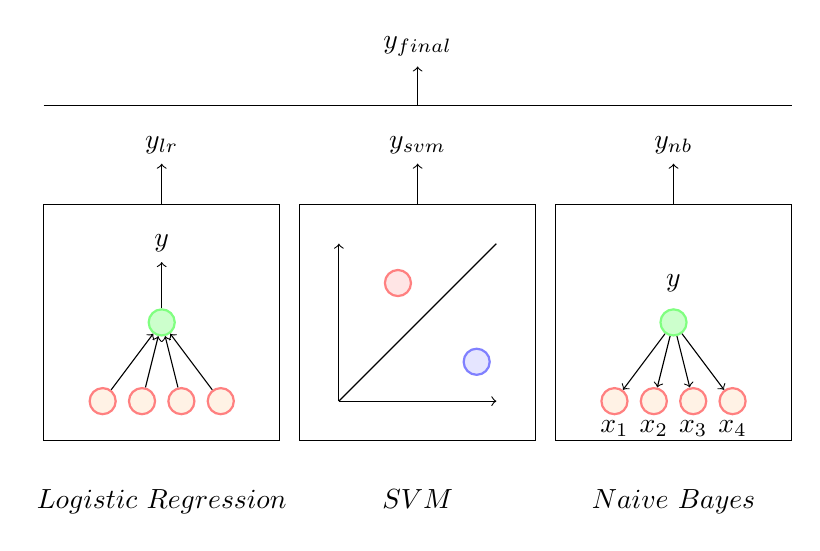
\begin{tikzpicture}
						
	\node [input_neuron] (in0) at (0.75,0.5) {};
	\node [input_neuron] (in1) at (1.25,0.5) {};
	\node [input_neuron] (in2) at (1.75,0.5) {} ;
	\node [input_neuron] (in3) at (2.25,0.5) {} ;
						
	\node [output_neuron] (out0) at (1.5,1.5)  {} ;
						
	\node (output0) at (1.5,2.5)  {$y$} ;
	\node (output1) at (1.5,3.75)  {$y_{lr}$} ;
	\draw (0,0) rectangle  (3,3);
	\draw [->] (in0) -- (out0);
	\draw [->] (in1) -- (out0);
	\draw [->] (in2) -- (out0);
	\draw [->] (in3) -- (out0);
	\draw [->] (out0) -- (output0);
	\draw [->] (1.5,3) -- (output1);
	\node [below] (head) at (1.5,-0.5)  {$Logistic$ $Regression$} ;
						
	\draw[->,xshift=0mm] (3.75,0.5) -- coordinate (x axis mid) (5.75,0.5);
	\draw[->,xshift=0mm] (3.75,0.5) -- coordinate (y axis mid)(3.75,2.5);
	\node [positive] (in0) at (4.5,2) {};
	\node [negative] (out0) at (5.5,1) {};
						
	\draw (3.25,0) rectangle  (6.25,3);
	\node (output2) at (4.75,3.75)  {$y_{svm}$} ;
	\draw [->] (4.75,3) -- (output2);
	\draw  (3.75,0.5) -- (5.75,2.5);
	\node [below] (head) at (4.75,-0.5)  {$SVM$} ;
						
	\draw (6.5,0) rectangle (9.5,3);
	\node (output3) at (8,3.75)  {$y_{nb}$} ;
	\draw [->] (8,3) -- (output3);
						
	\node [input_neuron] (in10) at (7.25,0.5) {};
	\node [input_neuron] (in11) at (7.75,0.5) {};
	\node [input_neuron] (in12) at (8.25,0.5) {} ;
	\node [input_neuron] (in13) at (8.75,0.5) {} ;
	\node at (7.25,0.15) {$x_1$};
	\node at (7.75,0.15) {$x_2$};
	\node at (8.25,0.15) {$x_3$};
	\node at (8.75,0.15) {$x_4$};
	\node [output_neuron] (out10) at (8,1.5)  {} ;
	\node (output0) at (8,2)  {$y$} ;
	\draw [->] (out10) -- (in10);
	\draw [->] (out10) -- (in11);
	\draw [->] (out10) -- (in12);
	\draw [->] (out10) -- (in13);
	\node [below] (head) at (8,-0.5)  {$Naive$ $Bayes$} ;
	\node (output3) at (4.75,5)  {$y_{final}$} ;
	\draw (0,4.25) -- (9.5,4.25);
	\draw [->] (4.75,4.25) -- (4.75,4.75);
\end{tikzpicture}
}
			}
		\end{overlayarea}
		\column{0.6\textwidth}
		\begin{overlayarea}{\textwidth}{\textheight}
			\begin{itemize}
				\justifying
							
				\item <1-> Combine the output of different models to reduce generalization error
				      \item<2->  The models can correspond to different classifiers
				      \item<3-> It could be different instances of the same classifier trained with:
				      \begin{itemize}
				      	\justifying
				      	\item<4-> different hyperparameters
				      	\item<5-> different features
				      	\item<6-> different samples of the training data
				      \end{itemize}
			\end{itemize}
		\end{overlayarea}
	\end{columns}
\end{frame}


\begin{frame}
	\begin{columns}
		\column{0.5\textwidth}
		\begin{overlayarea}{\textwidth}{\textheight}
					
			\only<1->{
						
\tikzstyle{input_neuron}=[circle,draw=red!50,fill=orange!10,thick,minimum size=.2mm]
\tikzstyle{hidden_neuron}=[circle,draw=blue!50,fill=blue!10,thick,minimum size=1mm]
\tikzstyle{output_neuron}=[circle,draw=green!50,fill=green!20,thick,minimum size=1mm]
\tikzstyle{output}=[circle,draw=green!50,fill=green!20,thick,minimum size=1mm]
\tikzstyle{positive}=[circle,draw=red!50,fill=red!10,thick,minimum size=.2mm]
\tikzstyle{negative}=[circle,draw=blue!50,fill=blue!10,thick,minimum size=1mm]
\resizebox{6cm}{5cm}{%
	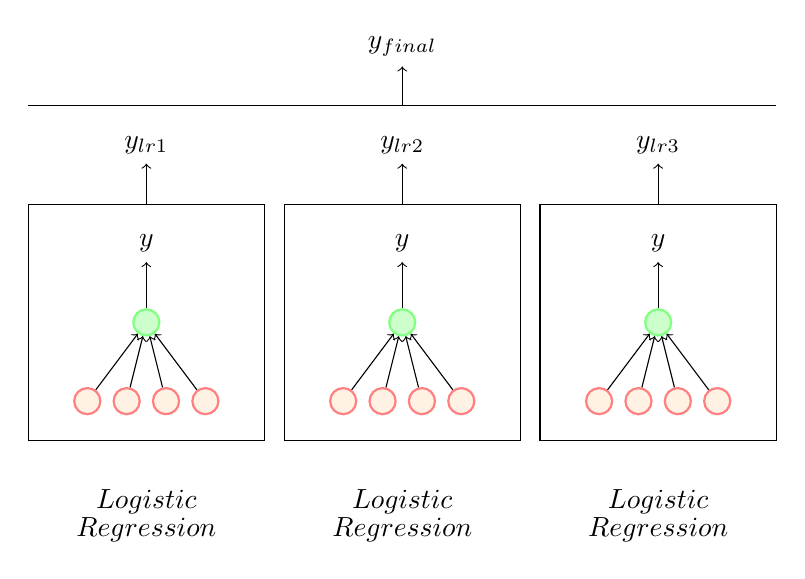
\begin{tikzpicture}
							
		\node [input_neuron] (in0) at (0.75,0.5) {};
		\node [input_neuron] (in1) at (1.25,0.5) {};
		\node [input_neuron] (in2) at (1.75,0.5) {} ;
		\node [input_neuron] (in3) at (2.25,0.5) {} ;
							
		\node [output_neuron] (out0) at (1.5,1.5)  {} ;
							
		\node (output0) at (1.5,2.5)  {$y$} ;
		\node (output1) at (1.5,3.75)  {$y_{lr1}$} ;
		\draw (0,0) rectangle  (3,3);
		\draw [->] (in0) -- (out0);
		\draw [->] (in1) -- (out0);
		\draw [->] (in2) -- (out0);
		\draw [->] (in3) -- (out0);
		\draw [->] (out0) -- (output0);
		\draw [->] (1.5,3) -- (output1);
						
							
		\node [input_neuron] (in4) at (4,0.5) {};
		\node [input_neuron] (in5) at (4.5,0.5) {};
		\node [input_neuron] (in6) at (5.0,0.5) {} ;
		\node [input_neuron] (in7) at (5.5,0.5) {} ;
							
		\node [output_neuron] (out1) at (4.75,1.5)  {} ;
							
		\node (output2) at (4.75,2.5)  {$y$} ;
		\node (output3) at (4.75,3.75)  {$y_{lr2}$} ;
		\draw (3.25,0) rectangle  (6.25,3);
		\draw [->] (in4) -- (out1);
		\draw [->] (in5) -- (out1);
		\draw [->] (in6) -- (out1);
		\draw [->] (in7) -- (out1);
		\draw [->] (out1) -- (output2);
		\draw [->] (4.75,3) -- (output3);
						
							
		\node [input_neuron] (in8) at (7.25,0.5) {};
		\node [input_neuron] (in9) at (7.75,0.5) {};
		\node [input_neuron] (in10) at (8.25,0.5) {} ;
		\node [input_neuron] (in11) at (8.75,0.5) {} ;
							
		\node [output_neuron] (out2) at (8,1.5)  {} ;
							
		\node (output4) at (8,2.5)  {$y$} ;
		\node (output5) at (8,3.75)  {$y_{lr3}$} ;
		\draw (6.5,0) rectangle (9.5,3);
		\draw [->] (in8) -- (out2);
		\draw [->] (in9) -- (out2);
		\draw [->] (in10) -- (out2);
		\draw [->] (in11) -- (out2);
		\draw [->] (out2) -- (output4);
		\draw [->] (8,3) -- (output5);
		\node [below] (head) at (4.75,-0.5)  {$Logistic$ } ;
		\node [below] (head) at (8,-0.5)  {$Logistic$ } ;
		\node [below] (head) at (1.5,-0.5)  {$Logistic$ } ;
		\node [below] (head) at (4.75,-0.85)  {$Regression$} ;
		\node [below] (head) at (8,-0.85)  { $Regression$} ;
		\node [below] (head) at (1.5,-0.85)  { $Regression$} ;
							
		\node (output3) at (4.75,5)  {$y_{final}$} ;
		\draw (0,4.25) -- (9.5,4.25);
		\draw [->] (4.75,4.25) -- (4.75,4.75);
	\end{tikzpicture}
}

				}
			\onslide<6->{Each model trained with a different sample of the data (sampling with replacement)}
		\end{overlayarea}
		\column{0.5\textwidth}
		\begin{overlayarea}{\textwidth}{\textheight}
			\begin{itemize}
				\justifying
				\item \onslide<3->  Bagging: form an ensemble using different instances of the same classifier
				\item \onslide<4-> From a given dataset, construct multiple training sets by sampling with replacement $(T_1, T_2, ... ,T_k)$
				\item \onslide<5-> Train $i^{th}$ instance of the classifier using training set $T_i$
			\end{itemize}
		\end{overlayarea}
	\end{columns}
\end{frame}

\begin{frame}
	\begin{columns}
		\column{0.5\textwidth}
		\begin{overlayarea}{\textwidth}{\textheight}
			\begin{itemize}
				\item <7-> The error made by the average prediction of all the models is $\frac{1}{k}\sum_{i}\varepsilon_i$
				\item <8-> The expected squared error is :
%				\vspace{-2cm}
				\scalebox{0.88}{\parbox{\linewidth}{%
					\begin{align*}
				 		%DeclareMathSizes{10}{10}{10}{10}
						\onslide<9-> {mse= & E[(\frac{1}{k}\sum_{i}\varepsilon_i)^{2}] \\} 
						\onslide<10-> {=   & \frac{1}{k^{2}}E[\sum_{i}\sum_{i=j} \varepsilon_i \varepsilon_j + \sum_{i}\sum_{i\neq j} \varepsilon_i \varepsilon_j] \\}
						\onslide<11-> {=   & \frac{1}{k^{2}}E[\sum_{i} \varepsilon_i^{2} + \sum_{i}\sum_{i\neq j} \varepsilon_i \varepsilon_j] \\}
						\onslide<12->{ =   & \frac{1}{k^{2}}(\sum_{i} E[\varepsilon_i^{2}] + \sum_{i}\sum_{i\neq j} E[\varepsilon_i \varepsilon_j]) \\}
						\onslide<13-> {=   & \frac{1}{k^{2}}(kV+k(k-1)C) \\}
						\onslide<14-> {=   & \frac{1}{k}V+\frac{k-1}{k}C  \\}
					\end{align*}
				}
			}
			% }
			\end{itemize}
		\end{overlayarea}
		\column{0.4\textwidth}
		\begin{overlayarea}{\textwidth}{\textheight}
			\begin{itemize}
				\justifying
				\item<1->  When would bagging work?
				\item<2-> Consider a set of $k$ LR models
				\item<3->  Suppose that each model makes an error $\varepsilon_i$ on a test example
				\item<4->  Let $\varepsilon_i$ be drawn from a zero mean multivariate normal distribution
				\item<5->  $ Variance = E[\varepsilon_i^{2}]=V$
				\item<6->  $Covariance = E[\varepsilon_i \varepsilon_j]=C$
			\end{itemize}
		\end{overlayarea}
	\end{columns}
\end{frame}


\begin{frame}
	\begin{columns}
		\column{0.5\textwidth}
		\begin{overlayarea}{\textwidth}{\textheight}
			\begin{equation*}
				mse=\frac{1}{k}V+\frac{k-1}{k}C
			\end{equation*}
		\end{overlayarea}
		\column{0.5\textwidth}
		\begin{overlayarea}{\textwidth}{\textheight}
			\begin{itemize}
				\justifying
				\item<2->  When would bagging work ?
				\item <3-> If the errors of the model are perfectly correlated then $V=C$ and $mse=V$ [bagging does not help: the mse of the ensemble is as bad as the individual models]
				\item<4->  If the errors of the model are independent or uncorrelated then $C=0$ and the mse of the ensemble reduces to $\frac{1}{k}V$
				\item <5-> On average, the ensemble will perform at least as well as its individual members
			\end{itemize}
		\end{overlayarea}
	\end{columns}
\end{frame}
